\documentclass{article}
\usepackage{amsmath}
\usepackage{amsfonts}

\usepackage{tikz}
\usetikzlibrary{fit,positioning,shapes}

\usepackage[shortlabels]{enumitem}

\usepackage{algorithm}
\usepackage{amssymb}
\usepackage{booktabs}
\usepackage{algpseudocode}

\textwidth=7.6in
\textheight=9.9in
\topmargin=-.9in
\headheight=0in
\headsep=.5in
\hoffset=-1.5in
\setlength\parindent{0pt}


\begin{document}

\begin{center}
    \Large{\textbf{Problem Set 2 Solutions}} \\[0.25ex]
    Calvin Walker
\end{center}
\textbf{1.}
\begin{enumerate}[(a)]
    \item \begin{align*}
        P(E) &= \sum_{r, m, h, s, b, a, l}P(r, m, h, s, b, a, l, E) \\ 
        &=  \sum_{r, m, h, s, b, a, l} P(r) P(m) P(h | r, m) P(s | h) P(a | h) P(b | h) P(E | s, b) P(l | b, a) \\
        &= \sum_{b}\sum_{s} P(E|s, b) \sum_{h} P(s | h) P(b | h) \sum_{a} P(a | h) \sum_{l} P(l | b, a) \sum_{r} P(r)\sum_{m} P(h | r, m) P(m)
    \end{align*}
    \item The corresponding elimination ordering is $\prec= M, R, L, A, H, S, B$
    \item \textcolor{white}{{x}}
    \begin{figure}[h]
        \centering
        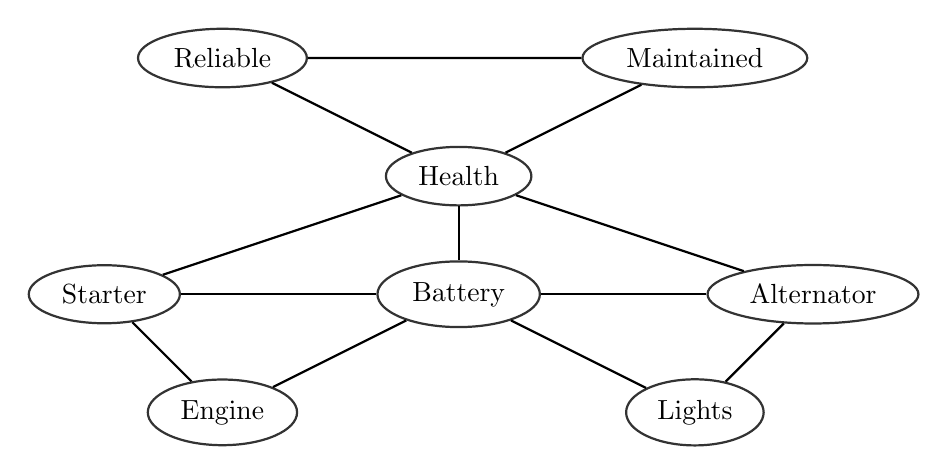
\begin{tikzpicture}[xscale=3.0,yscale=1.5]
            \tikzstyle{latent}=[ellipse, minimum size = 5mm, inner sep=4pt, thick, draw = black!80, node distance = 10mm]
            \tikzstyle{connect}=[thick]
            \node[latent] (R) at (-1,2){Reliable};
            \node[latent] (M) at (1,2){Maintained};
            \node[latent] (H) at (0,1){Health};
            \node[latent] (S) at (-1.5,0){Starter};
            \node[latent] (B) at (0,0){Battery};
            \node[latent] (A) at (1.5,0){Alternator};
            \node[latent] (E) at (-1,-1){Engine};
            \node[latent] (L) at (1,-1){Lights};
            \path[-] (R) edge [connect] (H);
            \path[-] (R) edge [connect] (M);
            \path[-] (S) edge [connect] (B);
            \path[-] (B) edge [connect] (A);
            \path[-] (M) edge [connect] (H);
            \path[-] (H) edge [connect] (S);
            \path[-] (H) edge [connect] (B);
            \path[-] (H) edge [connect] (A);
            \path[-] (S) edge [connect] (E);
            \path[-] (B) edge [connect] (E);
            \path[-] (B) edge [connect] (L);
            \path[-] (A) edge [connect] (L);
        \end{tikzpicture}
        \caption{Moralized graph for the Bayesian Network} \label{fig:auto-bn}
    \end{figure}
    \item The initial set of factors is $\Phi = \{\phi(H, M, R), \phi(S, B, H), \phi(H, B, A), \phi(S, B, E), \phi(B, A, L)\}$ 
    % Step 1: Eliminate $M$ \begin{enumerate}[(i)]
    %     \item $\psi_1(H, M, R) = \phi(H, M, R)$,  
    %     \item Variables involved: $H, M, R$
    %     \item $\tau_1(H, R)  = \sum_{m}\phi_1(H, m, R)$
    % \end{enumerate}
    \begin{table}[h!]
        \centering
        \begin{tabular}{|c|c|c|c|c|}
          \hline
        %   \multirow{2}{*}{Header 1} & \multicolumn{2}{c|}{Header 2} & \multirow{2}{*}{Header 3} & \multirow{2}{*}{Header 4} \\
          Step & Variable & Intermediate & Variables & New  \\
               & Eliminated & Factor & Involved & Factor \\
          \hline
          1 & $M$ & $\psi_1(H, M, R) = \phi(H, M, R)$ & $H, M, R$ & $\tau_1(H, R) = \sum_{m}\psi_1(H, m, R)$ \\
          2 & $R$ & $\psi_2(H, R) = \tau_1(H, R)$ & $H, R$ & $\tau_2(H) = \sum_{r}\psi_2(H, r)$ \\
          3 & $L$ & $\psi_3(B, A, L) = \phi(B, A, L)$ & $B, A, L$ & $\tau_3(B, A) = \sum_{l}\psi_3(B, A, l)$ \\
          4 & $A$ & $\psi_4(A, B, H) = \tau_3(B, A)\phi(H, B, A)$ & $H, B, A$ & $\tau_4(B, H) = \sum_{a}\psi_4(a, B, H)$ \\
          5 & $H$ & $\psi_5(S, B, H) = \tau_2(H)\tau_4(B, H)\phi(S, B, H)$ & $S, B, H$ & $\tau_5(S, B) = \sum_{h}\psi_5(S, B, h)$ \\
          6 & $B$ & $\psi_6(S, B, E) = \tau_5(S, B)\phi(S, B, E)$ & $S, B, E$ & $\tau_6(S, E) = \sum_{l}\psi_6(S, b, E)$ \\
          7 & $S$ & $\psi_6(S, E) = \tau_6(S, E)$ & $S, E$ & $\tau_7(E) = \sum_{s}\psi_7(s, E)$ \\
          \hline
        \end{tabular}
        \caption{Variable Elimination Procedure for $P(E)$}
        \label{tab:example}
      \end{table}
      \item The largest induced scope is $2$, and assuming each variable can take $k$ possible values, the computational complexity would be $O(nk^2)$, since the factor has $k^2$ entries. 
      \item The induced graph is the same as the moralized netowrk in part $(c)$, since there are already edges between all variables appearing in some $\psi$ generated by the variable elimination.
      \newpage
      \item \textcolor{white}{{x}}
      \begin{figure}[h]
        \centering
        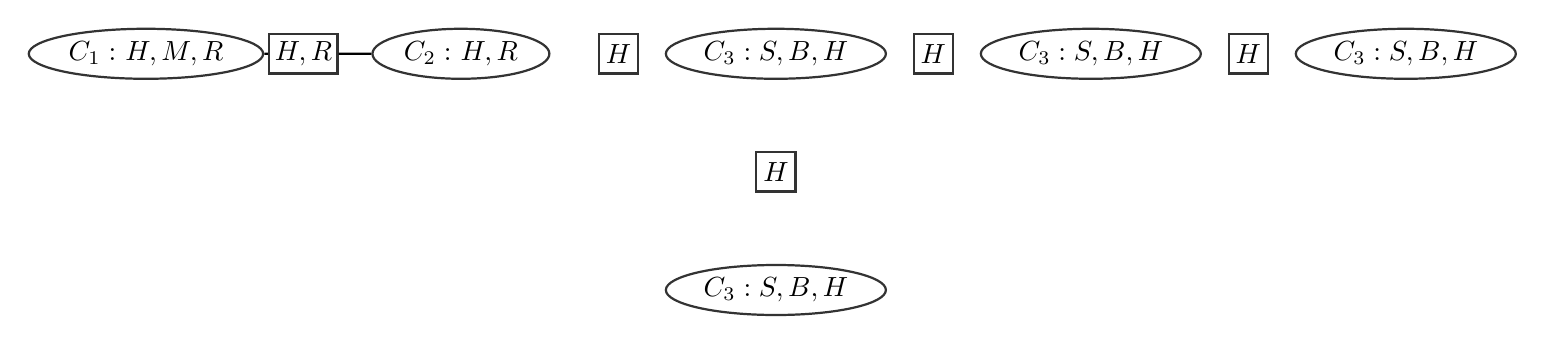
\begin{tikzpicture}[xscale=2.0,yscale=1.5]
            \tikzstyle{clique}=[ellipse, minimum size = 5mm, inner sep=2pt, thick, draw = black!80, node distance = 10mm]
            \tikzstyle{sepset}=[rectangle, minimum size = 5mm, inner sep=2pt, thick, draw = black!80, node distance = 10mm]
            \tikzstyle{connect}=[thick]
            \node[clique] (C1) at (-4,2){$C_1:$ $H, M, R$};
            \node[sepset] (S12) at (-3,2){$H, R$};
            \node[clique] (C2) at (-2,2){$C_2:$ $H, R$};
            \node[sepset] (S23) at (-1,2){$H$};
            \node[clique] (C3) at (0,2){$C_3:S, B, H$};
            \node[sepset] (S23) at (0,1){$H$};
            \node[clique] (C3) at (0,0){$C_3:S, B, H$};
            
            \node[sepset] (S23) at (1,2){$H$};
            \node[clique] (C3) at (2,2){$C_3:S, B, H$};
            \node[sepset] (S23) at (3,2){$H$};
            \node[clique] (C3) at (4,2){$C_3:S, B, H$};


            % \node[clique] (C2) at (-1,2){$C_1:$ $H, M, R$};
            % \node[latent] (M) at (1,2){Maintained};
            % \node[latent] (H) at (0,1){Health};
            % \node[latent] (S) at (-1.5,0){Starter};
            % \node[latent] (B) at (0,0){Battery};
            % \node[latent] (A) at (1.5,0){Alternator};
            % \node[latent] (E) at (-1,-1){Engine};
            % \node[latent] (L) at (1,-1){Lights};
            \path[-] (C1) edge [connect] (S12);
            \path[-] (S12) edge [connect] (C2);


        \end{tikzpicture}
        \caption{Moralized graph for the Bayesian Network}
    \end{figure}
      \item If we first eliminate $H$, there is an induced scope of $5$, as we create a new factor $\tau_1(R, M, S, B, A)$, next we could eliminate $B$, to induce a scope of $6$, as we create a new factor $\tau_2(R, M, S, A, E, L)$ with the remaining $6$ random variables. So any elimination ordering starting $\prec = H, B \dots$ would lead to a computational complexity of $O(nk^6)$
\end{enumerate}
\textbf{2.}
\end{document}